\documentclass[a4paper, 11pt]{article}

\usepackage[utf8]{inputenc}
\usepackage[portuguese]{babel}
\usepackage{indentfirst}
\usepackage[pdfborder={0 0 0}]{hyperref}
\usepackage{a4wide}
\usepackage{graphicx}
\usepackage{float}
\usepackage{fancyhdr}
\usepackage{lastpage}
\usepackage{listings}

\lstset{
    basicstyle=\small,
    numbers=left, 
    numberstyle=\tiny,
    numbersep=5pt,
    breaklines=true,
    frame=tB, 
    mathescape=true,
    escapeinside={(*@}{@*)},
    showstringspaces=false,
    captionpos=b
}

\title{Processamento de Linguagens \\  \Large Trabalho Prático nº 1}
\author{João Freitas (A83782) \and Luís Fernandes (A76712) \and Rui Fernandes (A89138)}
\date{Abril 2021}

\renewcommand{\labelitemi}{--}

\begin{document}

\begin{titlepage}
    \begin{center}
        \begin{minipage}{0.75\linewidth}
            \centering
            
\includegraphics[width=0.4\textwidth]{img/um_eeng.jpg}\par\vspace{1cm}
            \vspace{1.5cm}
            \href{https://www.uminho.pt/PT}{\scshape\LARGE Universidade do Minho} \par
            \vspace{1cm}
            \href{https://www.di.uminho.pt/}{\scshape\Large Departamento de Informática} \par
            \vspace{1.5cm}
            \maketitle
        \end{minipage}
    \end{center}
    \vspace{2cm}
    \thispagestyle{empty}
    \clearpage
\end{titlepage}

\pagenumbering{roman}

\begin{abstract}  
O presente relatório descreve o trabalho prático realizado no âmbito da disciplina de
\href{https://miei.di.uminho.pt/plano_estudos.html#processamento_de_linguagens}
{\emph{Processamento de Linguagens}}, ao longo do segundo semestre do terceiro ano do
\href{http://miei.di.uminho.pt}{Mestrado Integrado em Engenharia Informática} da
\href{https://www.uminho.pt}{Universidade do Minho}.

A realização deste trabalho prático tem como principal objetivo o processamento de um ficheiro XML
de forma a extrair todos os dados considerados relevantes, ficheiro esse que contém o registo de
rapazes que pretendiam seguir a vida clerical e se candidatavam aos seminários. O processamento deste
ficheiro será feito através de Expressões Regulares para a descrição de padrões de frases dentro de
textos.

Neste documento descrevemos sucintamente o programa desenvolvido e discutimos as decisões tomadas
durante a realização do trabalho prático.
\end{abstract}

\pagebreak

\tableofcontents

\listoffigures

\pagebreak

\pagenumbering{arabic}

\pagestyle{fancy}
\fancyhf{}

\rfoot{Página \thepage \hspace{1pt} de \pageref{LastPage}}

\renewcommand{\headrulewidth}{0pt}

\section{Introdução}
\label{sec:introducao}

\subsection{Enquadramento e Contexto}

Os \textit{Róis de Confessados} são arquivos do arcebispado existentes no Arquivo Digital de Braga que
contém o registo de rapazes que pretendiam seguir a vida clerical e se candidatavam aos seminários,
contendo milhares de registos. Cada um desses registos contém informação relativa ao nome do candidato
e dos seus pais, assim como eventuais parentes que apadrinhem a sua candidatura.

O trabalho apresentado tem como objetivo usar o módulo \texttt{re} da linguagem \texttt{Python} para
filtrar um conjunto de dados fornecidos, extraindo desses dados a informação relevante.

Adicionalmente, recorrendo ao módulo \texttt{pyplot} da biblioteca \texttt{matplotlib}, assim como à
biblioteca \texttt{graphviz}, foi possível gerar alguns gráficos que permitem uma melhor visualização
dos dados, tal como será apresentado na secção \ref{sec:testes}.

\subsection{Problema e Objetivo}

Dado um ficheiro XML com alguns milhares de registos relativos a candidaturas aos seminários
pretende-se desenvolver um programa em \texttt{Python} de modo a:

\begin{itemize}
    \item Calcular o número de processos por ano;
    \item Calcular a frequência de nomes próprios e apelidos;
    \item Calcular o número de candidatos que têm parentes eclesiásticos;
    \item Verificar se mesmo pai ou a mesma mãe têm mais do que um filho candidato;
    \item Desenhar todas as árvores genealógicas dos candidatos referentes a um determinado ano.
\end{itemize}

Desta forma, numa primeira fase, o problema passa por limpar e normalizar todos estes registos. Em
seguida,  será  necessário criar estruturas de dados adequadas para armazenar esta informação para
processá-la posteriormente.

\section*{Estrutura do Relatório}

O presente relatório encontra-se dividido em 4 partes.

No capítulo \ref{sec:introducao}, Introdução, é feito um enquadramento e contextualização do trabalho
prático e, em
seguida, é feita uma descrição do problema. 

No capítulo \ref{sec:solucao}, Concepção da Solução, são expostas as estruturas de dados utilizadas
e é feita uma descrição detalhada de todo o desenvolvimento do projeto até se obter a solução final.

De seguida, no capítulo \ref{sec:testes}, Codificação e Testes, são apresentados alguns testes
realizados e os resultados obtidos.

Por fim, no capítulo \ref{sec:conclusao}, Conclusão, termina-se o relatório com uma síntese a análise
crítica do trabalho desenvolvido.

\pagebreak

\section{Concepção da Solução}
\label{sec:solucao}

Dado um ficheiro XML com milhares de registos, é necessário extrair de cada candidatura toda a informação
relevante e, posteriormente, inseri-la em estruturas de dados adequadas.

A seguir apresenta-se um exemplo da forma como um processo é representado. Note-se, no entanto, que
alguns destes campos podem estar em falta.

\

\begin{lstlisting}
  <processo id="13123">
    <pasta>569</pasta>
    <data>1869-12-02</data>
    <nome>Abilio Augusto Santos</nome>
    <pai>Jose Joaquim Santos</pai>
    <mae>Teresa Jesus</mae>
    <obs>Antonio Jose Adao,Tio Materno. Proc.12530. Albino Antonio Ribeiro,Primo Paterno. Proc.12721.</obs>
  </processo>
\end{lstlisting}

\subsection{Estruturas de Dados}

Para conseguirmos armazenar temporariamente a informação relativa a uma candidatura, existiu a
necessidade de construir uma estrutura de dados que nos permitisse guardar os diferentes atributos.
Nesse sentido, foi criada a classe \texttt{Processo}, que tem todas as variáveis necessárias para guardar
a informação de uma candidatura.

\

\begin{lstlisting}[language=Python]
class Processo:
    def __init__(self, id, data, nome, pai, mae, obs):
        self.id = id
        self.data = data
        self.nome = nome
        self.pai = pai
        self.mae = mae
        self.obs = obs
        
    def __eq__(self, o: object) -> bool:
        return self.__class__ == o.__clcaptionpos=bass__ and self.id == o.id and self.data == o.data and self.nome == o.nome and \
               self.pai == o.pai and self.mae == o.mae and self.obs == o.obs

    def __hash__(self) -> int:
        return hash(self.id)
\end{lstlisting}

\

De forma a processar o ficheiro XML contendo a informação relativa aos processos, foi desenvolvida
uma função \texttt{parse\_xml} responsável por ler o ficheiro, instanciar os processos como objetos
da classe \texttt{Processo} e, posteriormente, adicioná-los a um dicionário. Este dicionário, em que
cada século está associado um outro dicionário no qual a cada ano corresponde uma lista contendo os
processos relativos a esse ano, permite um fácil acesso aos processos de um determinado intervalo de
tempo.

Note-se que uma vez que existem entradas repetidas no ficheiro XML, estas foram removidas de forma a
não tornar o resultado redundante.

\

\begin{lstlisting}[language=Python]
def remove_duplicates(processos_dict):
    for (sec, anos_dict) in processos_dict.items():
        for (ano, _) in anos_dict.items():
            processos_dict[sec][ano] = list(set(processos_dict[sec][ano]))
    return processos_dict


def parse_xml(lines):
    processos_dict = {}
    processos_XML = re.search(r'<processos>\s*(<processo id[\S\s]*</processo>)\s*</processos>', lines)
    processos = re.findall(r'<processo id[\S\s]*?</processo>', processos_XML.group(1))
    for p in processos:
        id = re.search(r'<processo id="(\d+)">', p).group(1)
        data = re.search(r'<data>(\d{4}-\d{2}-\d{2})</data>', p).group(1)
        nome = re.search(r'<nome>(.*)</nome>', p).group(1)
        pai = re.search(r'<pai>([\w\s]*),?\w*</pai>', p)
        if pai:
            pai = pai.group(1)
        else:
            pai = ''
        mae = re.search(r'<mae>([\w\s]*),?\w*</mae>', p)
        if mae:
            mae = mae.group(1)
        else:
            mae = ''
        obs = re.search(r'<obs>(.*)</obs>', p)
        if obs:
            obs = obs.group(1)
        else:
            obs = ''

        ano = int(data[:4])
        seculo = ano // 100 + 1

        if seculo not in processos_dict.keys():
            processos_dict[seculo] = {}

        try:
            processos_dict[seculo][ano].append(Processo(id, data, nome, pai, mae, obs))
        except KeyError:
            processos_dict[seculo][ano] = []
            processos_dict[seculo][ano].append(Processo(id, data, nome, pai, mae, obs))

    return remove_duplicates(processos_dict)
\end{lstlisting}

\subsection{Algoritmos}

\subsubsection{Alínea a}

Estando todos os processos já inseridos em dicionários organizado por séculos e anos, para determinar
quantos processos existem em cada ano basta calcular o tamanho da lista de processos relativa a esse
ano. Em relação ao número de séculos, devolve-se o tamanho do dicionário que, por sua vez, contém os
dicionários relativos a cada um dos anos.

Por outro lado, para determinar o intervalo de datas em que há registos, começa-se por determinar a
menor chave do dicionário de séculos, que corresponde ao menor século, e, com essa chave, determina-se
a menor chave do dicionário de anos associado a essa chave, que corresponde ao menor ano. Por fim,
tendo a lista de processos associada a esse ano, basta ordenar a lista tendo em conta a data de cada
um dos processos. Desta forma, a data o primeiro processo corresponderá, então, à data do primeiro
registo.

Num processo idêntico, para determinar a data do último registo calcula-se a maior chave do dicionário
de séculos e, posteriormente, determina-se a maior chave do dicionário de anos associado a essa chave,
que corresponderá ao maior ano. Assim, ordenando a lista tendo em consideração a data de cada um dos
processos, basta verificar qual a data do processo mais recente.


\begin{lstlisting}[language=Python]
def alinea_a(processos_dict):
    x = []
    y = []

    for anos_dict in sorted(processos_dict.values(), key=lambda item: sorted(item)):
        for (ano, p) in sorted(anos_dict.items()):
            print(f'{ano}: {len(p)} processos')
            x.append(ano)
            y.append(len(p))
    print(f'Foram analisados {len(processos_dict)} seculos')

    min_seculo = min(processos_dict.keys())
    min_ano = min(processos_dict[min_seculo].keys())
    min_date = sorted(processos_dict[min_seculo][min_ano], key=lambda p: p.data)[0].data

    max_seculo = max(processos_dict.keys())
    max_ano = max(processos_dict[max_seculo].keys())
    max_date = sorted(processos_dict[max_seculo][max_ano], key=lambda p: p.data, reverse=True)[0].data

    print(f'Existem processos entre {min_date} e {max_date}')

    plt.style.use('seaborn')
    plt.bar(x, y, linestyle='solid', color='green')
    plt.title('Numero de Processos por Ano')
    plt.ylabel('Numero de Processos')
    plt.xlabel('Ano')
    plt.gcf().autofmt_xdate()
    plt.tight_layout()
    plt.show()
\end{lstlisting}

\subsubsection{Alínea b}

Para determinar a frequência global de nomes próprios e apelidos, itera-se sobre todos os processos
guardados e para cada nome no processo guarda-se o primeiro nome como chave num dicionário tendo como
valor a contagem atual desse nome. Este processo é repetido para o último nome do titular do processo,
noutro dicionário.

\

\begin{lstlisting}[language=Python]
def alinea_b(processos_dict):
    nomes_proprios = {}
    apelidos = {}

    for (sec, anos_dict) in processos_dict.items():
        for (ano, proc) in anos_dict.items():
            for p in proc:
                nome = re.split(r'\s+', p.nome)
                nome_proprio = nome[0]
                apelido = nome[-1]
                try:
                    nomes_proprios[nome_proprio] += 1
                except KeyError:
                    nomes_proprios[nome_proprio] = 1
                try:
                    apelidos[apelido] += 1
                except KeyError:
                    apelidos[apelido] = 1

    print('GLOBAL')
    print('\nNomes Proprios\n')
    for (nome, freq) in list(sorted(nomes_proprios.items(), key=lambda item: item[1], reverse=True)):
        print(f'{nome} -> {freq}')
    print('\nApelidos\n')
    for (nome, freq) in list(sorted(apelidos.items(), key=lambda item: item[1], reverse=True)):
        print(f'{nome} -> {freq}')

    print('\nPOR SECULO')
    for sec in sorted(processos_dict.keys()):
        print(f'\nSeculo {sec}')
        (nome, apelido) = nome_apelido_seculo(sec, processos_dict)
        print(f'Nomes: {", ".join([x[0] for x in nome])}')
        print(f'Apelidos: {", ".join([x[0] for x in apelido])}')
\end{lstlisting}

\pagebreak

Além disso, para obter os 5 nomes próprios e apelidos mais frequentes em cada um dos séculos, repete-se
a iteração sobre os processos, mas desta vez apenas considerando os referentes a cada século, e são
retornados os 5 nomes e apelidos mais frequentes.

\

\begin{lstlisting}[language=Python]
def nome_apelido_seculo(seculo, processos_dict):
    nomes_proprios = {}
    apelidos = {}
    for proc in processos_dict[seculo].values():
        for p in proc:
            nome = re.split(r'\s+', p.nome)
            nome_proprio = nome[0]
            apelido = nome[-1]
            try:
                nomes_proprios[nome_proprio] += 1
            except KeyError:
                nomes_proprios[nome_proprio] = 1
            try:
                apelidos[apelido] += 1
            except KeyError:
                apelidos[apelido] = 1
    nome = list(sorted(nomes_proprios.items(), key=lambda item: item[1], reverse=True))[:5]
    apelido = list(sorted(apelidos.items(), key=lambda item: item[1], reverse=True))[:5]
    return nome, apelido
\end{lstlisting}

\pagebreak

\subsubsection{Alínea c}

Para calcular o número de candidatos com parentes eclesiásticos (irmão, tio ou primo), itera-se sobre
todos os processos e no campo relativo às observações de cada um dos processo são procuradas todas
as ocorrências das palavras irmão, tio ou primo, através de expressões regulares. Caso existam ocorrências,
é incrementado o contador de candidatos com parentes eclesiásticos, assim como o contador da respetiva
ocorrência do grau de parentesco. Por fim, é retornado o número de candidatos com parentes eclesiásticos
bem como o parentesco mais frequente.

\

\begin{lstlisting}[language=Python]
def alinea_c(processos_dict):
    parentes = {'Irmao': 0, 'Tio': 0, 'Primo': 0}
    r = 0
    for (sec, anos_dict) in processos_dict.items():
        for (ano, proc) in anos_dict.items():
            for p in proc:
                tem_parente = False
                if irmaos := re.findall(r'(?i:irmaos?)', p.obs):
                    parentes['Irmao'] += len(irmaos)
                    tem_parente = True
                if tios := re.findall(r'(?i:tio)', p.obs):
                    parentes['Tio'] += len(tios)
                    tem_parente = True
                if primos := re.findall(r'(?i:primo)', p.obs):
                    parentes['Primo'] += len(primos)
                    tem_parente = True
                if tem_parente:
                    r += 1
    print(f'{r} candidatos tem parentes eclesiasticos')
    print(
        f'O grau de parentesco mais comum e {list(sorted(parentes.items(), key=lambda item: item[1], reverse=True))[0][0]}')

    x = list(parentes.keys())
    y = list(parentes.values())
    plt.style.use('seaborn')
    plt.bar(x, y, linestyle='solid', color='green')
    plt.title('Grau de Parentesco Mais Comum')
    plt.xlabel('Grau de Parentesco')
    plt.ylabel('Frequencia')
    plt.tight_layout()
    plt.show()
\end{lstlisting}

\pagebreak

\subsubsection{Alínea d}

De modo a verificar se o mesmo pai ou a mesma mãe têm mais do que um filho candidato, itera-se sobre
todos os processos  e incrementa-se o valor de um contador caso o progenitor do titular do processo
em questão corresponda ao nome pretendido. Quando for encontrado mais do que um processo cujo titular
seja descendente do parente em questão, a iteração termina. Caso contrário, a iteração continua e, caso
o ciclo termine, conclui-se, então, que o progenitor tem, no máximo, um filho candidato à vida clerical.

\

\begin{lstlisting}[language=Python]
def alinea_d_pai(pai, processos_dict):
    n = 0
    for (sec, anos_dict) in processos_dict.items():
        for (ano, proc) in anos_dict.items():
            for p in proc:
                if p.pai == pai:
                    n += 1
                    if n > 1:
                        print(f'{pai} tem mais do que um filho candidato')
                        return
    print(f'{pai} nao tem mais do que um filho candidato')


def alinea_d_mae(mae, processos_dict):
    n = 0
    for (sec, anos_dict) in processos_dict.items():
        for (ano, proc) in anos_dict.items():
            for p in proc:
                if p.mae == mae:
                    n += 1
                    if n > 1:
                        print(f'{mae} tem mais do que um filho candidato')
                        return
    print(f'{mae} nao tem mais do que um filho candidato')
\end{lstlisting}

\pagebreak

\subsubsection{Alínea e}

Para construir todas as árvores genealógicas referentes a um determinado ano, itera-se sobre todos
os processos referentes a esse mesmo ano e, com base na linguagem de desenho de grafos \texttt{DOT},
desenham-se nodos para o titular do processo e para os progenitores, assim como um arco entre eles.
Note-se, no entanto, que alguns dos processos não possuem informação relativa a um dos progenitores.

Por fim, recorrendo à biblioteca \texttt{graphviz}, é possível visualizar o grafo gerado.

\

\begin{lstlisting}[language=Python]
def alinea_e(ano, processos_dict):
    seculo = ano // 100 + 1
    f = open('arvore_genealogica.dot', 'w')
    f.write('digraph arvore_genealogica {\n')
    try:
        for p in processos_dict[seculo][ano]:
            if p.mae:
                f.write(f'\t{p.mae.replace(" ", "")} -> {p.nome.replace(" ", "")};\n')
            if p.pai:
                f.write(f'\t{p.pai.replace(" ", "")} -> {p.nome.replace(" ", "")};\n')
        f.write('}\n')
        f.close()
        src = Source.from_file('arvore_genealogica.dot')
        src.view()
    except KeyError:
        print('Nao existe informacao sobre esse ano')

\end{lstlisting}

\pagebreak

\section{Codificação e Testes}
\label{sec:testes}

\subsection{Testes realizados e Resultados}

Ao longo da realização do trabalho prático fomos testando os métodos elaborados através de diferentes
testes.  Mostram-se a seguir alguns testes feitos e os respetivos resultados obtidos.

\

\subsubsection{Alínea a}

\begin{figure}[H]
    \centering
    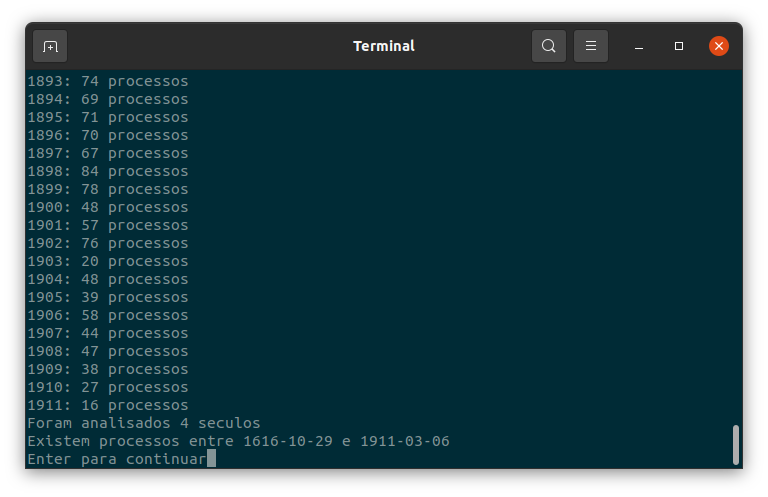
\includegraphics[width=.9\textwidth]{img/a.png}
    \caption{Número de processos por ano}
\end{figure}

\pagebreak

Adicionalmente, com o intuito de perimitir uma melhor visualização dos dados, e fazendo uso do módulo
\texttt{pyplot} da biblioteca \texttt{matplotlib}, foram gerados alguns gráficos que se apresentam
de seguida.

\begin{figure}[H]
    \centering
    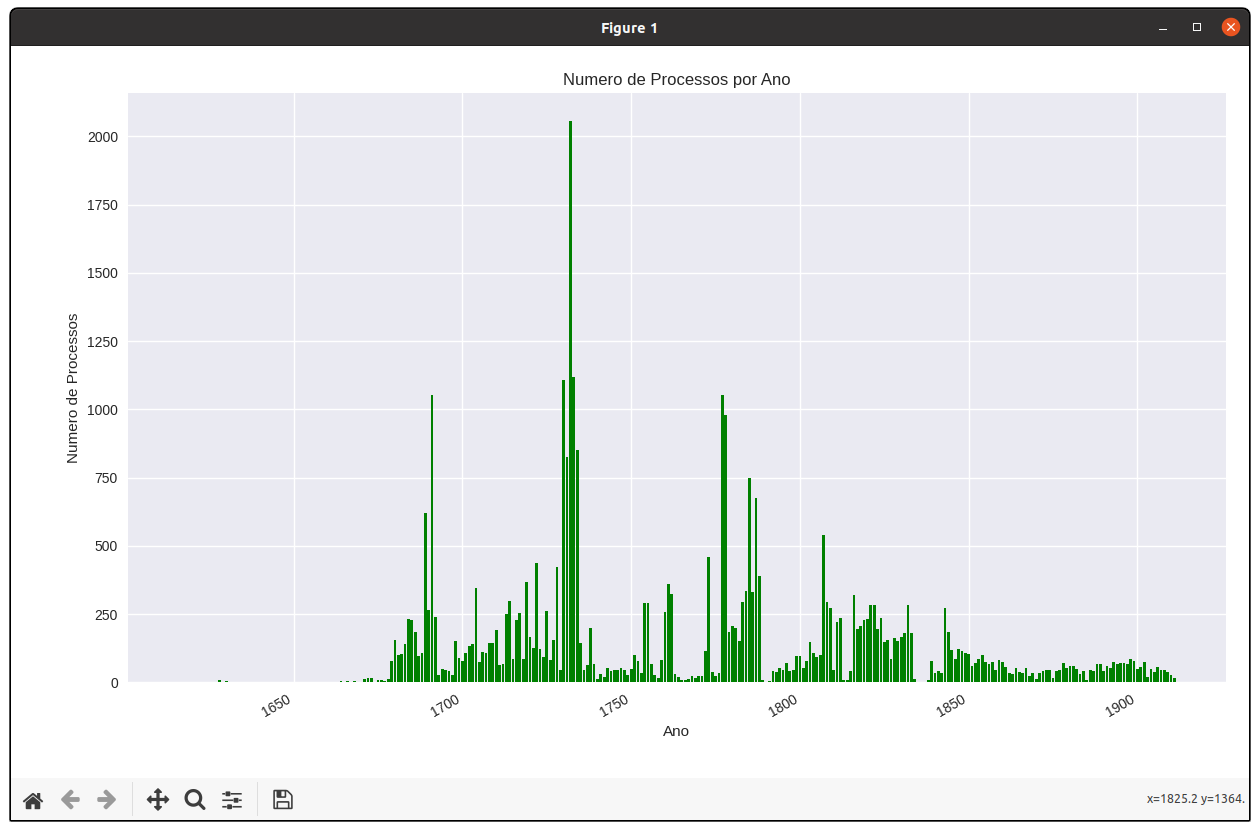
\includegraphics[width=.8\textwidth]{img/m1.png}
    \caption{Número de processos por ano}
\end{figure}

\begin{figure}[H]
    \centering
    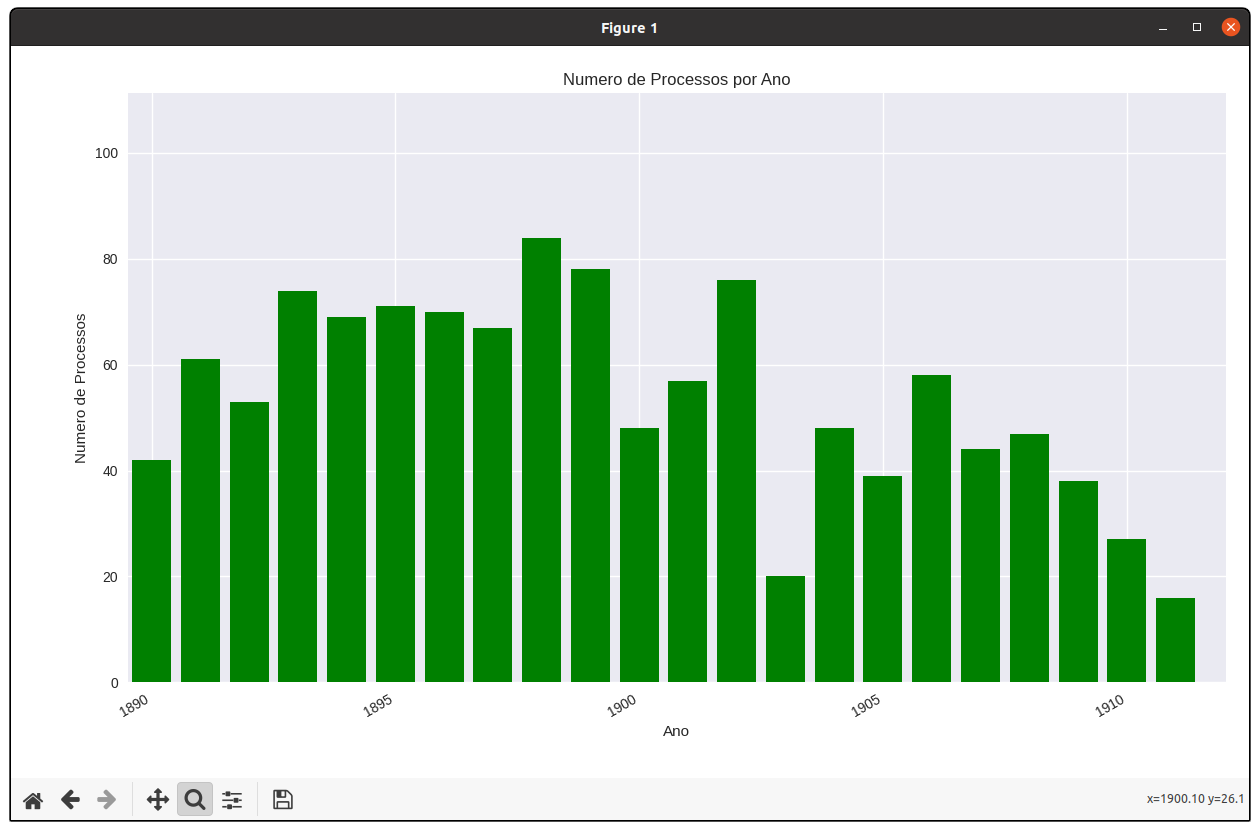
\includegraphics[width=.8\textwidth]{img/m2.png}
    \caption{Número de processos por ano, num intervalo de tempo}
\end{figure}

\subsubsection{Alínea b}

\begin{figure}[H]
    \centering
    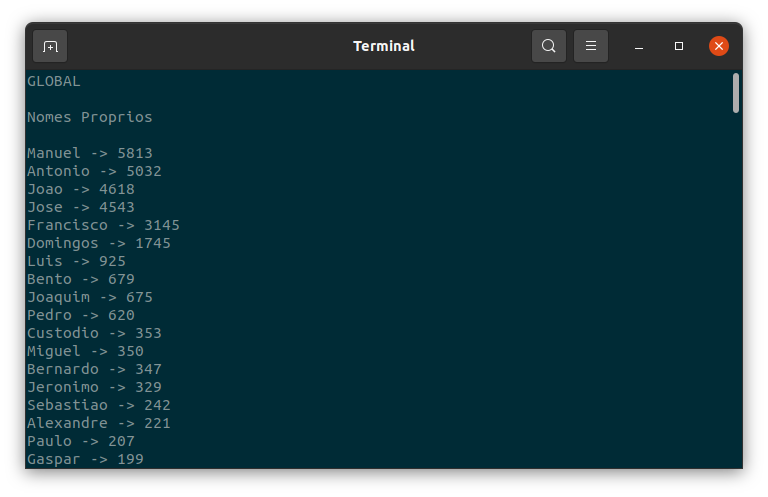
\includegraphics[width=.8\textwidth]{img/nomes.png}
    \caption{Frequência global de nomes próprios}
\end{figure}

\begin{figure}[H]
    \centering
    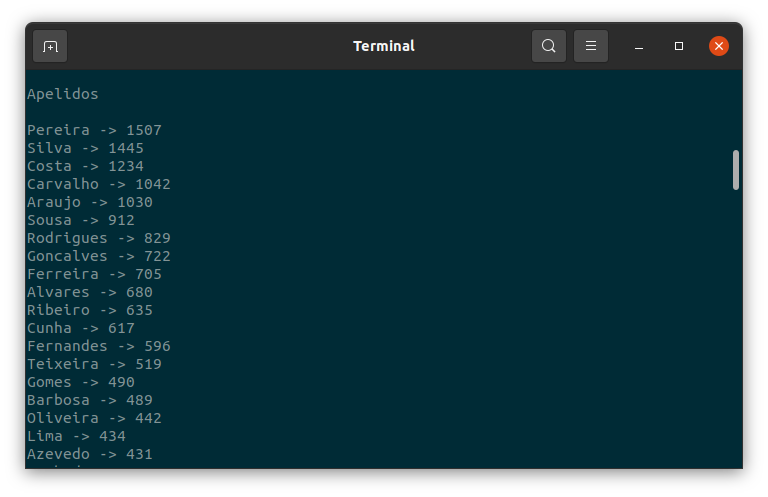
\includegraphics[width=.8\textwidth]{img/apelidos.png}
    \caption{Frequência global de apelidos}
\end{figure}

\begin{figure}[H]
    \centering
    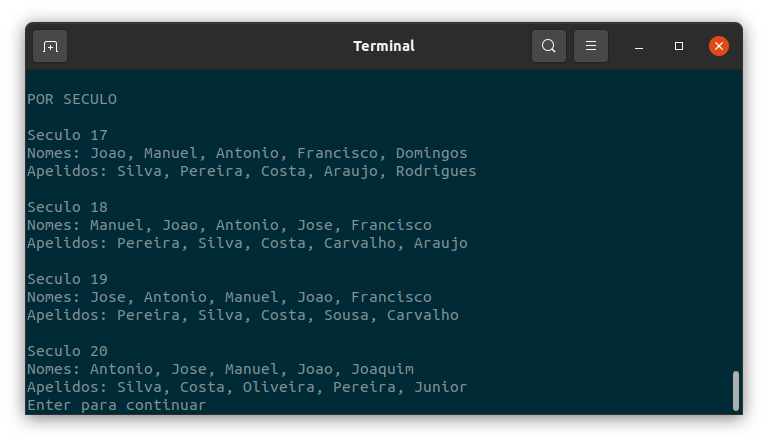
\includegraphics[width=.8\textwidth]{img/b.png}
    \caption{Nomes próprios e apelidos mais comuns em cada século}
\end{figure}

\subsubsection{Alínea c}

\begin{figure}[H]
    \centering
    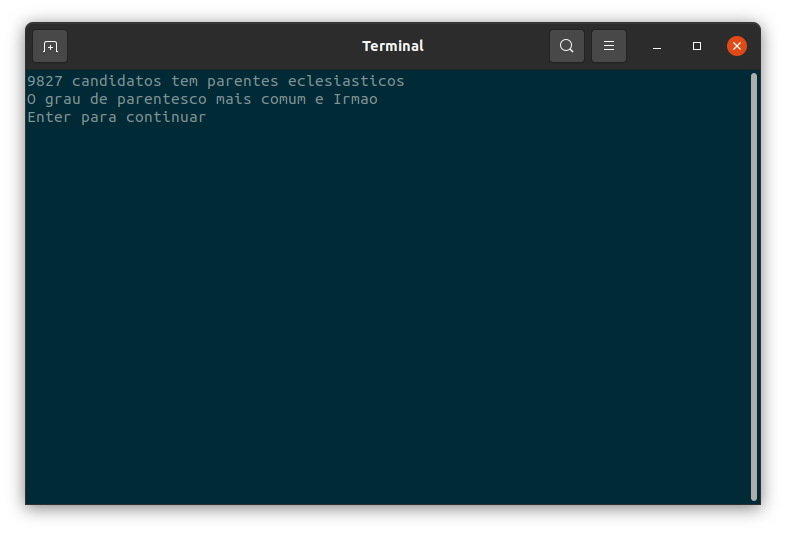
\includegraphics[width=.8\textwidth]{img/c1.png}
    \caption{Número de candidatos com parentes eclesiásticos}
\end{figure}

\begin{figure}[H]
    \centering
    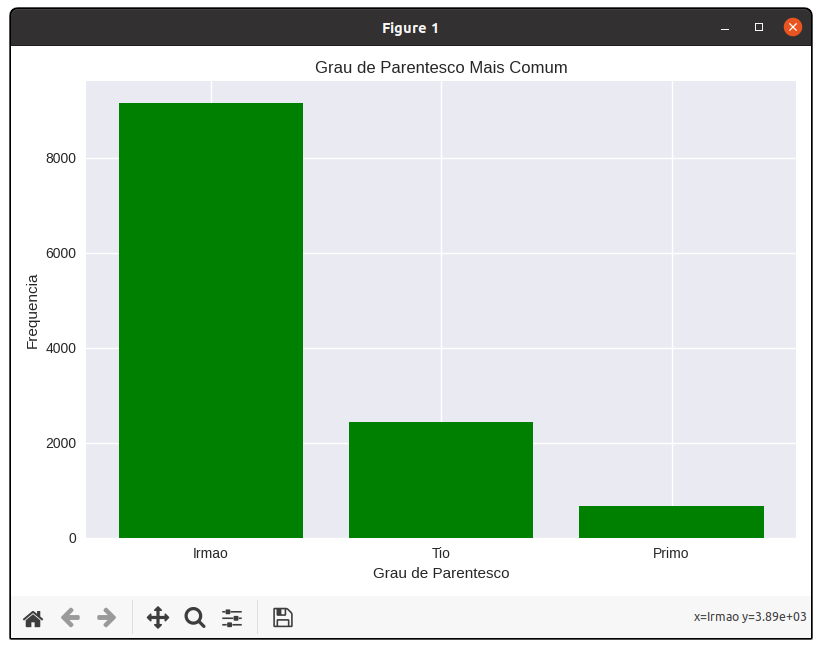
\includegraphics[width=.8\textwidth]{img/c2.png}
    \caption{Graus de parentesco e respetiva frequência}
\end{figure}

\subsubsection{Alínea d}

\begin{figure}[H]
    \centering
    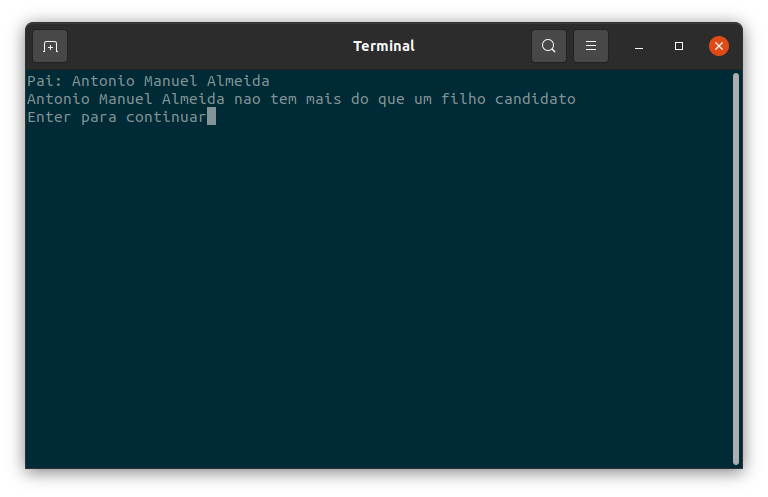
\includegraphics[width=.8\textwidth]{img/pai.png}
    \caption{Pai com no máximo um filho candidato}
\end{figure}

\begin{figure}[H]
    \centering
    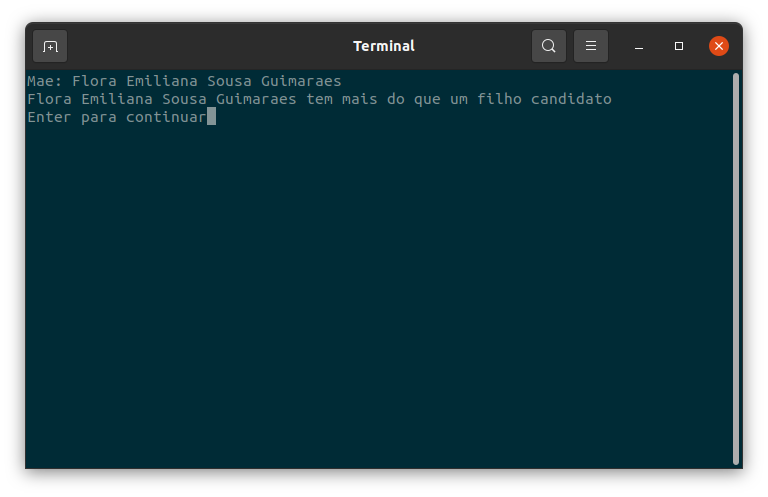
\includegraphics[width=.8\textwidth]{img/mae.png}
    \caption{Mãe com mais do que um filho candidato}
\end{figure}

\subsubsection{Alínea e}

De seguida apresentam-se as árvores genealógicas dos candidatos referentes ao ano de 1836, assim como
o ficheiro \texttt{.dot} gerado:

\

\begin{lstlisting}
digraph arvore_genealogica {
    JacintaMaria -> BernardoCunhaBrochado;
    AntonioCunhaBrochado -> BernardoCunhaBrochado;
    LuisaTeixeira -> AlvaroAfonsoTavares;
    ManuelAfonsoTavares -> AlvaroAfonsoTavares;
}
\end{lstlisting}

\

\begin{figure}[H]
    \centering
    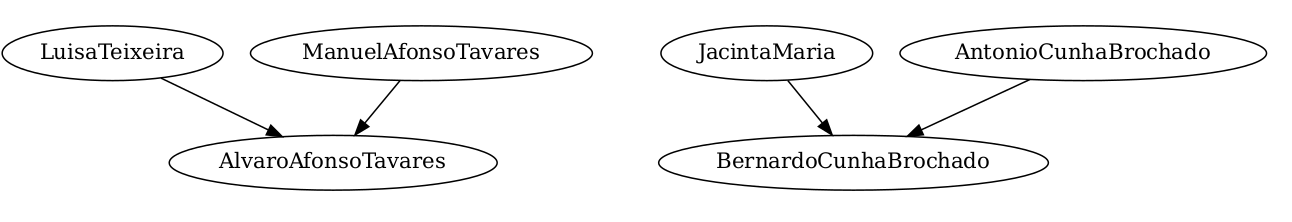
\includegraphics[width=\textwidth]{img/1836.png}
    \caption{Árvores genealógicas dos candidatos referentes ao ano de 1836}
\end{figure}

\pagebreak

\section{Conclusão}
\label{sec:conclusao}

Através do desenvolvimento deste projeto conseguimos aumentar a capacidade relativamente à escrita
de expressões regulares como motor para a filtração e transformação de textos. 

Fazendo uma análise geral ao trabalho desenvolvido, fazemos um balanço bastante positivo do trabalho
realizado, conseguindo atingir todos os requisitos propostos. A utilização de Expressões Regulares
para o tratamento de \textit{strings} mostrou-se um mecanismo extremamente poderoso, permitindo
simplificar tarefas que de outra forma seriam consideravelmente mais complexas e demoradas.

Com o resultado final do projeto e na perspetiva do grupo, pensa-se que se atingiu da melhor forma
todos os objetivos propostos e sempre pensando na simplicidade e descomplicação do problema. De facto,
foi possível responder a todas as questões, bem como acrescentar algumas funcionalidades extra que
consideramos serem relevantes. 

\end{document}
